\documentclass[14pt]{extbook}
\usepackage{multicol, enumerate, enumitem, hyperref, color, soul, setspace, parskip, fancyhdr} %General Packages
\usepackage{amssymb, amsthm, amsmath, latexsym, units, mathtools} %Math Packages
\everymath{\displaystyle} %All math in Display Style
% Packages with additional options
\usepackage[headsep=0.5cm,headheight=12pt, left=1 in,right= 1 in,top= 1 in,bottom= 1 in]{geometry}
\usepackage[usenames,dvipsnames]{xcolor}
\usepackage{dashrule}  % Package to use the command below to create lines between items
\newcommand{\litem}[1]{\item#1\hspace*{-1cm}\rule{\textwidth}{0.4pt}}
\pagestyle{fancy}
\lhead{Progress Quiz 4}
\chead{}
\rhead{Version B}
\lfoot{5346-5907}
\cfoot{}
\rfoot{Summer C 2021}
\begin{document}

\begin{enumerate}
\litem{
Choose the graph of the equation below.\[ f(x) = \frac{-1}{(x + 1)^2} + 2 \]\begin{enumerate}[label=\Alph*.]
\begin{multicols}{2}\item 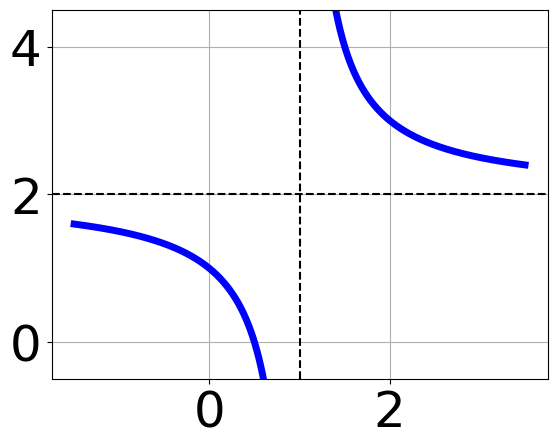
\includegraphics[width = 0.3\textwidth]{../Figures/rationalEquationToGraphAB.png}\item 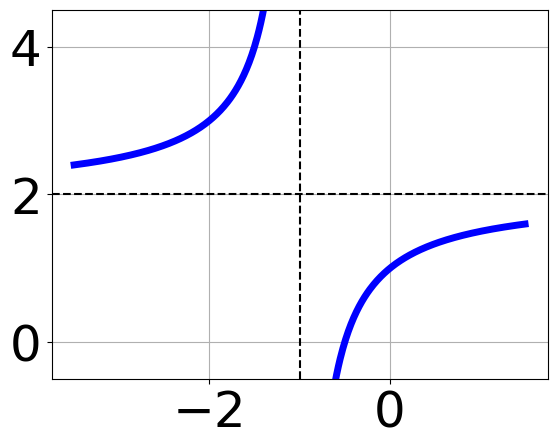
\includegraphics[width = 0.3\textwidth]{../Figures/rationalEquationToGraphBB.png}\item 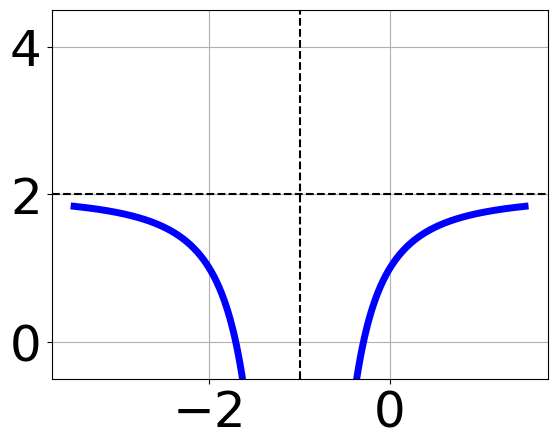
\includegraphics[width = 0.3\textwidth]{../Figures/rationalEquationToGraphCB.png}\item 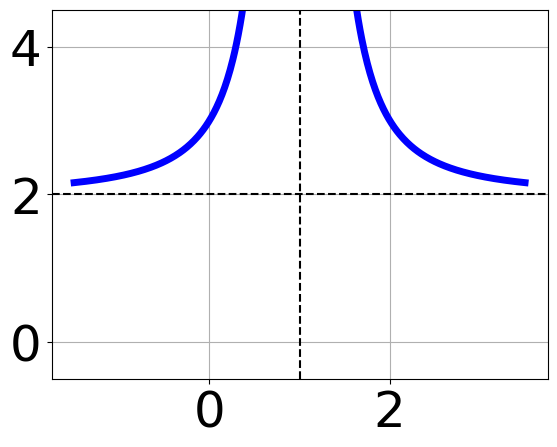
\includegraphics[width = 0.3\textwidth]{../Figures/rationalEquationToGraphDB.png}\end{multicols}\item None of the above.
\end{enumerate} }
\litem{
Choose the equation of the function graphed below.
\begin{center}
    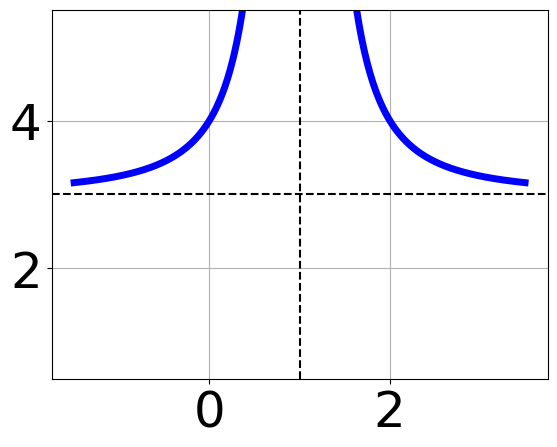
\includegraphics[width=0.5\textwidth]{../Figures/rationalGraphToEquationCopyB.png}
\end{center}
\begin{enumerate}[label=\Alph*.]
\item \( f(x) = \frac{1}{(x - 1)^2} + 3 \)
\item \( f(x) = \frac{1}{x - 1} + 3 \)
\item \( f(x) = \frac{-1}{x + 1} + 3 \)
\item \( f(x) = \frac{-1}{(x + 1)^2} + 3 \)
\item \( \text{None of the above} \)

\end{enumerate} }
\litem{
Choose the equation of the function graphed below.
\begin{center}
    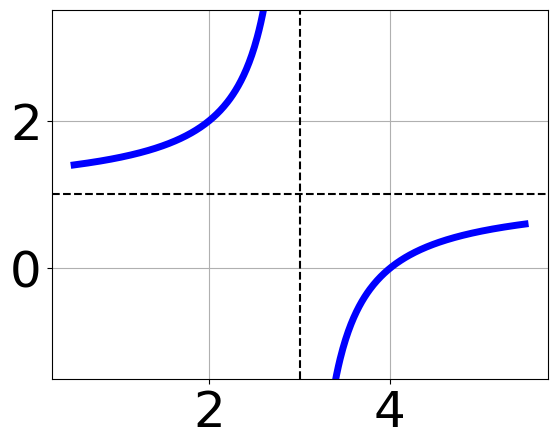
\includegraphics[width=0.5\textwidth]{../Figures/rationalGraphToEquationB.png}
\end{center}
\begin{enumerate}[label=\Alph*.]
\item \( f(x) = \frac{-1}{x - 3} + 1 \)
\item \( f(x) = \frac{-1}{(x - 3)^2} + 1 \)
\item \( f(x) = \frac{1}{x + 3} + 1 \)
\item \( f(x) = \frac{1}{(x + 3)^2} + 1 \)
\item \( \text{None of the above} \)

\end{enumerate} }
\litem{
Solve the rational equation below. Then, choose the interval(s) that the solution(s) belongs to.\[ \frac{-56}{-35x -14} + 1 = \frac{-56}{-35x -14} \]\begin{enumerate}[label=\Alph*.]
\item \( x \in [-0.4,0.6] \)
\item \( x_1 \in [-1.3, -0.3] \text{ and } x_2 \in [0.2,1.2] \)
\item \( \text{All solutions lead to invalid or complex values in the equation.} \)
\item \( x \in [0.3,1.6] \)
\item \( x_1 \in [-1.3, -0.3] \text{ and } x_2 \in [-1.5,-0.1] \)

\end{enumerate} }
\litem{
Solve the rational equation below. Then, choose the interval(s) that the solution(s) belongs to.\[ \frac{-7x}{2x -3} + \frac{-5x^{2}}{12x^{2} -24 x + 9} = \frac{-4}{6x -3} \]\begin{enumerate}[label=\Alph*.]
\item \( x \in [-0.77,0.63] \)
\item \( x_1 \in [0.55, 1.03] \text{ and } x_2 \in [-0.16,0.48] \)
\item \( \text{All solutions lead to invalid or complex values in the equation.} \)
\item \( x_1 \in [0.82, 2.19] \text{ and } x_2 \in [0.46,0.85] \)
\item \( x \in [0.82,2.19] \)

\end{enumerate} }
\litem{
Determine the domain of the function below.\[ f(x) = \frac{5}{20x^{2} -5 x -25} \]\begin{enumerate}[label=\Alph*.]
\item \( \text{All Real numbers except } x = a, \text{ where } a \in [-25, -23] \)
\item \( \text{All Real numbers except } x = a, \text{ where } a \in [-1, 1] \)
\item \( \text{All Real numbers.} \)
\item \( \text{All Real numbers except } x = a \text{ and } x = b, \text{ where } a \in [-25, -23] \text{ and } b \in [19, 23] \)
\item \( \text{All Real numbers except } x = a \text{ and } x = b, \text{ where } a \in [-1, 1] \text{ and } b \in [1.25, 2.25] \)

\end{enumerate} }
\litem{
Solve the rational equation below. Then, choose the interval(s) that the solution(s) belongs to.\[ \frac{5}{-4x -2} + -7 = \frac{3}{36x + 18} \]\begin{enumerate}[label=\Alph*.]
\item \( x \in [0.1,1.4] \)
\item \( x_1 \in [-0.8, -0.2] \text{ and } x_2 \in [-0.4,2.1] \)
\item \( x_1 \in [-0.8, -0.2] \text{ and } x_2 \in [-0.8,0.2] \)
\item \( x \in [-0.69,0.31] \)
\item \( \text{All solutions lead to invalid or complex values in the equation.} \)

\end{enumerate} }
\litem{
Solve the rational equation below. Then, choose the interval(s) that the solution(s) belongs to.\[ \frac{4x}{2x + 2} + \frac{-7x^{2}}{-12x^{2} -6 x + 6} = \frac{-4}{-6x + 3} \]\begin{enumerate}[label=\Alph*.]
\item \( \text{All solutions lead to invalid or complex values in the equation.} \)
\item \( x \in [0.69,0.98] \)
\item \( x_1 \in [-0.64, 0.28] \text{ and } x_2 \in [-1.7,-0.8] \)
\item \( x \in [-0.08,0.57] \)
\item \( x_1 \in [-0.64, 0.28] \text{ and } x_2 \in [-0.8,1.7] \)

\end{enumerate} }
\litem{
Choose the graph of the equation below.\[ f(x) = \frac{1}{x - 3} - 1 \]\begin{enumerate}[label=\Alph*.]
\begin{multicols}{2}\item 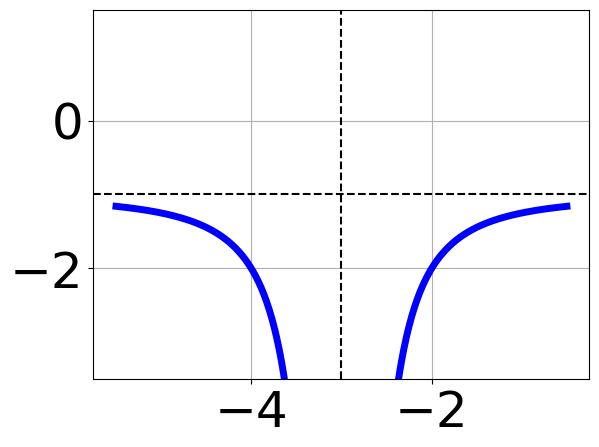
\includegraphics[width = 0.3\textwidth]{../Figures/rationalEquationToGraphCopyAB.png}\item 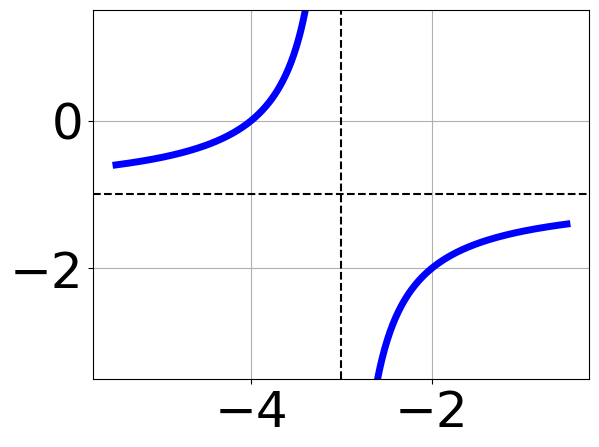
\includegraphics[width = 0.3\textwidth]{../Figures/rationalEquationToGraphCopyBB.png}\item 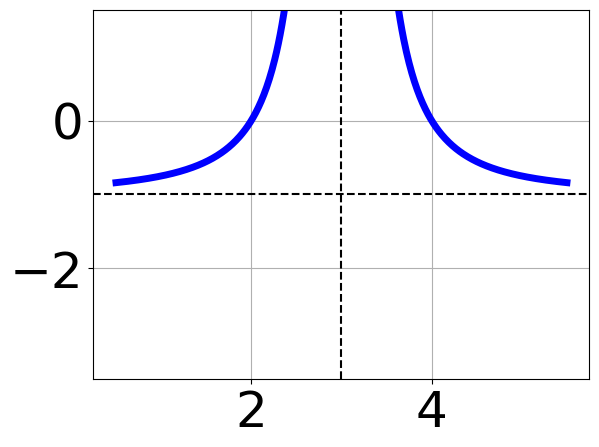
\includegraphics[width = 0.3\textwidth]{../Figures/rationalEquationToGraphCopyCB.png}\item 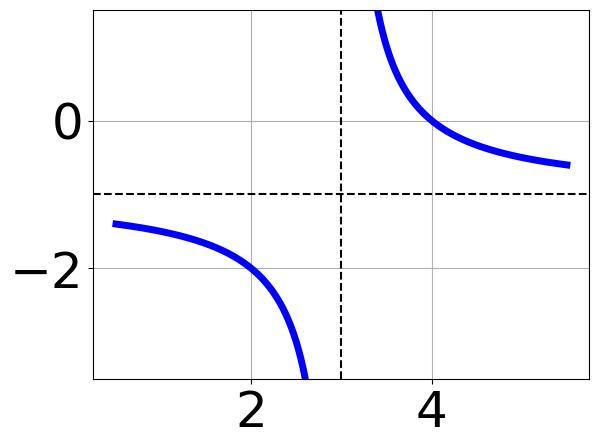
\includegraphics[width = 0.3\textwidth]{../Figures/rationalEquationToGraphCopyDB.png}\end{multicols}\item None of the above.
\end{enumerate} }
\litem{
Determine the domain of the function below.\[ f(x) = \frac{5}{20x^{2} +9 x -20} \]\begin{enumerate}[label=\Alph*.]
\item \( \text{All Real numbers except } x = a, \text{ where } a \in [-2.25, -0.25] \)
\item \( \text{All Real numbers except } x = a \text{ and } x = b, \text{ where } a \in [-2.25, -0.25] \text{ and } b \in [0.8, 3.8] \)
\item \( \text{All Real numbers.} \)
\item \( \text{All Real numbers except } x = a, \text{ where } a \in [-20, -19] \)
\item \( \text{All Real numbers except } x = a \text{ and } x = b, \text{ where } a \in [-20, -19] \text{ and } b \in [17, 24] \)

\end{enumerate} }
\end{enumerate}

\end{document}